\documentclass{ctexart}
%
%页眉页脚
\usepackage{geometry}
\geometry{left=2.5cm,right=2.5cm,top=2.5cm,bottom=2.5cm}
\usepackage{xcolor}
\usepackage{graphicx}
\usepackage{amsmath}
\usepackage{url}
\usepackage{enumerate}
\usepackage{subfigure}
\usepackage{listings}
\usepackage[colorlinks,linkcolor=black]{hyperref}%书签
\usepackage{fancyhdr}

\fancyhead[R]{\thepage}%这是奇数页右页眉、偶数页左页眉
\fancyhead[L]{}
\chead{全球导航卫星系统基础}%这是中间页眉
\pagestyle{fancy}
\lstset{
    extendedchars=false, %解决代码跨页时,章节标题,页眉等汉字不显示的问题
    xleftmargin=1.5em,xrightmargin=1.5em, aboveskip=1em, %设置边距
    language=Matlab,
    basicstyle = \footnotesize,
    breaklines,
    captionpos = t,
    commentstyle = \color[rgb]{0,0.5,0},
    frameshape = {RYRYNYYYY}{yny}{yny}{RYRYNYYYY},
    keywordstyle = \color{blue}\bfseries,
    numbers = left,
    numberstyle = \tiny\color[rgb]{0.5,0.5,0.5},
    showstringspaces = false,
    stringstyle = \color[rgb]{0.58,0,0.82},
    tabsize = 4,
    title = \lstname
}
%中文
\usepackage{xeCJK}
%字体设置
\usepackage{enumitem}
\usepackage{indentfirst}
\setlength{\parindent}{2em}%首行缩进
\renewcommand\thesubsection{\alph{subsection}}
\renewcommand\thesubsubsection{\alph{subsubsection}}
\CTEXsetup[format={\Large\bfseries}]{section}

\title{第一次大作业P1:卫星位置计}
\author{聂浩(2013011280)}
\date{\today}
\begin{document}
\maketitle
\section{以GPS或其它导航系统为例,通过查阅文献等方式,调研其星历 有效期,星历更新方式(给出参考文献)}; 
目前, GPS卫星星历的提供方式有广播星历、超快速星历 (IGU星历)、快速星历(IGR星历)和精密星历(IGS 星历)4种类型。

在实际的接收机应用中一般使用广播星历,广播星历,是通过卫星发射的含有轨道信息的导航电文,每个卫星广播的星历每2h更新一次,即有效时间为两小时,或在用户距离误差(URE)超过规定限值时更新,其精度大约为3m\footnote{IGS超快速星历预推GPS卫星轨道精度分析,张耀文,贾小林,杨志强}。

其他的三种星历由IGS组织(International GPS service)发布\footnote{GPS星历、在轨描述和位置算法,刘基余}发布,其中IGS星历的精度最高,发布约在12d后,采样间隔15min,每周更新。

\section{根据其ICD文档编写卫星轨道计算程序,并下载一段星历,计算 卫星在其有效期内的卫星位置; }
使用星历为shao1520.16n\footnote{下载自\url{ftp://cddis.gsfc.nasa.gov/gps/data/daily/2016/152/16n/}},其为2016年5月31日的星历,计算中选取2:00:00,10号卫星的星历参数,所得结果为[ -12443.60, 10746.30, -20825.70],单位为km,对应wgs84的ecef坐标系。

根据精确星历igs18992.sp3\footnote{下载自\url{ftp://cddis.gsfc.nasa.gov/gps/products/1889/}}可以读出此时卫星的精确位置为[-12464.247088,10697.922314,-20838.267391]。可见存在一定的误差

计算代码为如下,执行方式为sat(2,0)。
\lstinputlisting{sat.m}

\section{星历有效性分析:假定星历有效期为T(小时),试计算2T、5T、 1天、5天、10天、20天以后(或以前)卫星位置,并分别与利用有效 期内星历计算所得卫星位置进行比较,通过定量比较,分析星历有效性}

由于目前在6月5日之后的igs数据无法查询到,故用igu数据代替,根据igs18992.sp3,igs18993.sp3,igu19001\_00.sp3,igu19006\_00.sp3,igu19021\_00.sp3读出10号卫星的位置,将利用上一问的方法得到的数据与实际位置进行比较,计算其之间的距离,得到如图\ref{bijiao},各个时间节点的误差距离分别为[54.08,8.92,5.54,57.20,4819.60,4809.80,9223.29],单位为km,可以看出,在5T内误差基本在同一数量级内,在1d后误差迅速扩大,使得预测失去意义。

代码如下
\lstinputlisting{draw.m}
\begin{figure}
    \centering
    % Requires \usepackage{graphicx}
    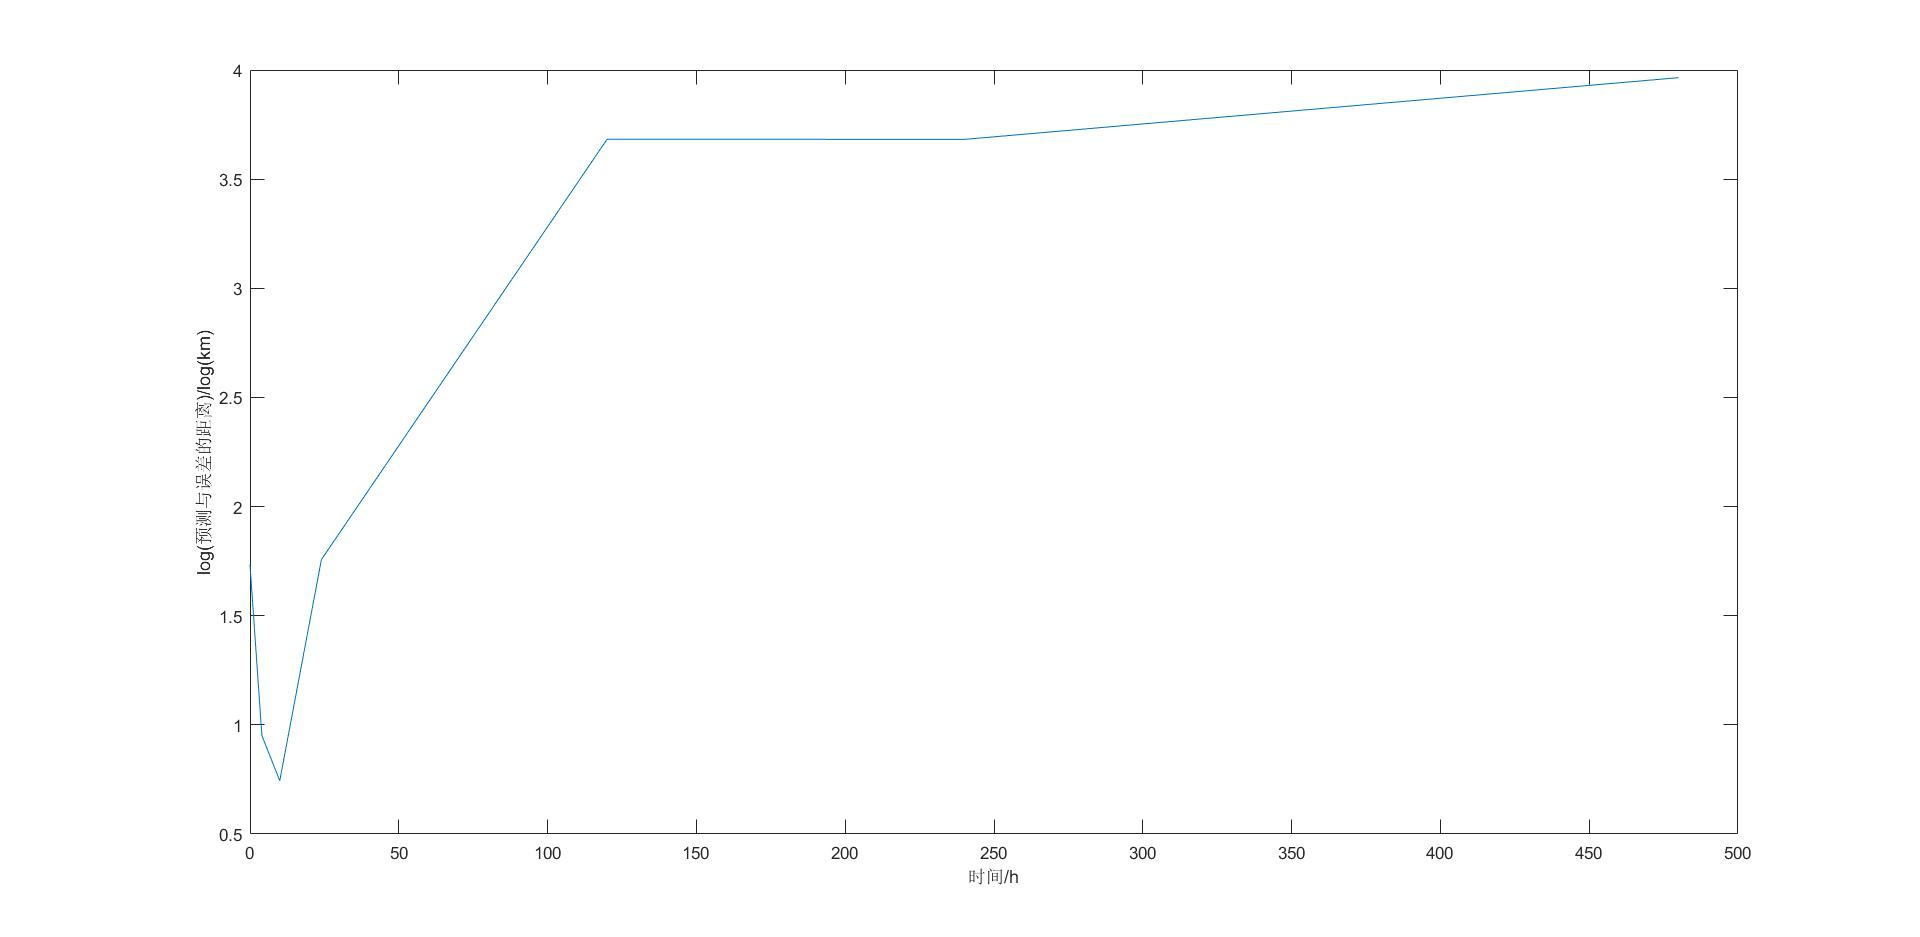
\includegraphics[width=0.8\textwidth]{pic/时间与运算精度.jpg}\\
    \caption{时间与预测误差}
    \label{bijiao}
\end{figure}
\end{document}
